\documentclass[a4paper, amsfonts, amssymb, amsmath, reprint, showkeys, nofootinbib, twoside]{revtex4-1}
\usepackage[english]{babel}
\usepackage[utf8]{inputenc}
\usepackage[colorinlistoftodos, color=green!40, prependcaption]{todonotes}
\usepackage[pdftex, pdftitle={Article}, pdfauthor={Author}]{hyperref}
\usepackage{amsthm}
\usepackage{mathtools}
\usepackage{physics}
\usepackage{xcolor}
\usepackage{caption}
\usepackage{hyperref}
%\hypersetup{colorlinks=true, linkcolor=blue, urlcolor = blue}
\usepackage{amsmath}
\usepackage{amssymb}
\usepackage{graphicx}
\graphicspath{Images}
\usepackage[left=23mm,right=13mm,top=35mm,columnsep=15pt]{geometry} 
\usepackage{adjustbox}
\usepackage{placeins}
\usepackage[T1]{fontenc}
\usepackage{float}
%\usepackage{longtable}
\usepackage{csquotes}
\usepackage{refstyle}
\usepackage{lipsum}

\begin{document}

\title{Millikan's Oil drop Experiment to determine the charge of electron.}
\author{Swaroop Ramakant Avarsekar}
\email{swaroop.avarsekar@niser.ac.in}
\affiliation{School of Physical Sciences, National Institute of Science Education and Research, HBNI, Jatni -752050, India}
\date{\today}

	
\begin{abstract}
Two methods are used to determine the charge of electron by Millikan's oil drop experiment, dynamic method and balancing method. In dynamic method the oil droplet is allowed free fall and then to rise in electric field; by calculating the time taken to rise and fall, with the working formula derived from various forces such as buoyant force, gravitational, electric, viscous force etc.. acting on the droplet during this process, e can be determined. In case of balancing method, the droplet is kept stationary with the help of certain potential difference to cancel out other forces acting on it. From dynamic method, we found charge of electron as $(4.706\pm0.095)\times10^{-19} C$ and with balancing method we found charge of electron as $(2.076\pm0.028)\times10^{-19} C$, hereby concluding from our experiment that charge is quantized; balancing method proved to be better in determining e.
\end{abstract}
	
\keywords{Viscosity, Quantisation, Charge}
	
\maketitle

\section{Introduction and Theory}
Millikan was the first person to determine the charge on electron winning to Nobel Prize in Physics in 1923. The setup consisted of horizontal separated parallel plates, with opening on the upper plate through which microscopic oil droplets are allowed to fall by gravitational field. By Stokes law, we can calculate the mass of the droplets and radii of the oil if density of oil is known. This method is called Dynamic method. In dynamic method, gravitational force, along with buoyant and viscous force come into the picture with former dominating than latter.By applying a potential difference between the plates, measuring velocity, by noting the time taken to travel certain distance, allows calculation of electric force on the droplets due to charge carried by them. This method is called balancing method. In this method, electric force and buoyant force cancels the viscous force and gravitational force. The charges on the droplets are caused due to friction. Moreover, this experiment will also prove that the charge on electron is quantized.  

Consider a spherical droplet of radius r, density $\rho$ under free fall. This will reach a terminal velocity of acted by constant force, $F_\eta=6\pi r\eta v_f$ where $\eta$ is coeffiecient of viscosity of air and $v_f$ is terminal velocuty . Graviational and buoyant force acta balanceed by $F_\eta$ where $\rho_a$ is density of air.
\begin{equation}
	4\pi r^3\rho g/3 -4\pi r^3\rho_a g/3=6\pi r\eta v_f
\end{equation}
\begin{equation}
	v_f=2g r^2(\rho  -\rho_a) /9\eta
\end{equation}
If the droplet has charge $n.e$ and moving upward with terminal velocity $v_f$ with electric field, V/d where V is the potential difference between the plates separated by distance $d$. 

\begin{equation}
	4\pi r^3(\rho  -\rho_a)/3+6\pi r\eta v_r=Vne/d
\end{equation} 
Subtracting equation (1) and (3), 
\begin{equation}
	ne=6\pi r\eta d(v_f+v_r)
\end{equation}

Dividing equation 4 by 2, we get
\begin{equation}
	ne=\frac{4\pi}{3V} gd(\rho  -\rho_a)r^3\left( 1+\frac{v_r}{v_f}\right) 
\end{equation}

The expression falling velocity $v_f$ on after correction due to the fact that the radii of droplets are of order micron which is less than mean free path of air molecules, resulting droplets falling quickly in free space between air molecules.

\begin{equation}
	v_f=\frac{2g r^2(\rho  -\rho_a)} {9\eta}\left( 1+\frac{c}{Pr}\right) 
\end{equation}

where c=6.17$\times10^{-8}$ mmHg is correction factor and P is the atmospheric pressure in mHg
Let 
\begin{equation}
\xi=\frac{9\eta v_f}{2g(\rho  -\rho_a)}
\end{equation}

\begin{equation}
	\zeta=\frac{c}{2P}
\end{equation}

Therefore, equation (6) converts to 
\begin{equation}
	r^2+2\zeta r-\xi=0
\end{equation}

Radius of droplet is given by
\begin{equation}
	r=-\zeta+\sqrt{\zeta^2+\xi}
\end{equation}

Equation (5) is used for dynamic method and for balancing method, with $V_b$ as balancing potential  we have,
\begin{equation}
	ne=\frac{4\pi gd(\rho-\rho_a)r^3}{3V_b}
\end{equation}

\section{Experiment}
\subsection{Apparatus}
The setup consists of oil drop chamber where two plates are separated by small distance. a CCD camera is placed to view the image of oil droplets passing connected to a LCD monitor. The plates are supplied with the voltage ranging from 0-800 V. A stopwatch to measure time taken by droplet to fall a specific distance. An atomizer is used to spray oil droplets.

\subsection{Procedure}
Fix two equidistant lines on the LCD display. Spray the oil droplets from atomizer. Two methods will be used to calculate the charge on the electron, one being Dynamic and other being Balancing method. In dynamic method, we measure the time taken by the medium sized droplet to under free fall certain distance marked on the display, and by applying voltage, as the the rise time of droplet is also calculated. Several measurements are repeated. In balancing method a certain voltage is applied to the droplet so that droplet is balanced by various forces acting on it and remains stationery. Voltage may have to be adjusted time to time.

\begin{figure}[H] %  figure placement: here, top, bottom, or page
	\centering
	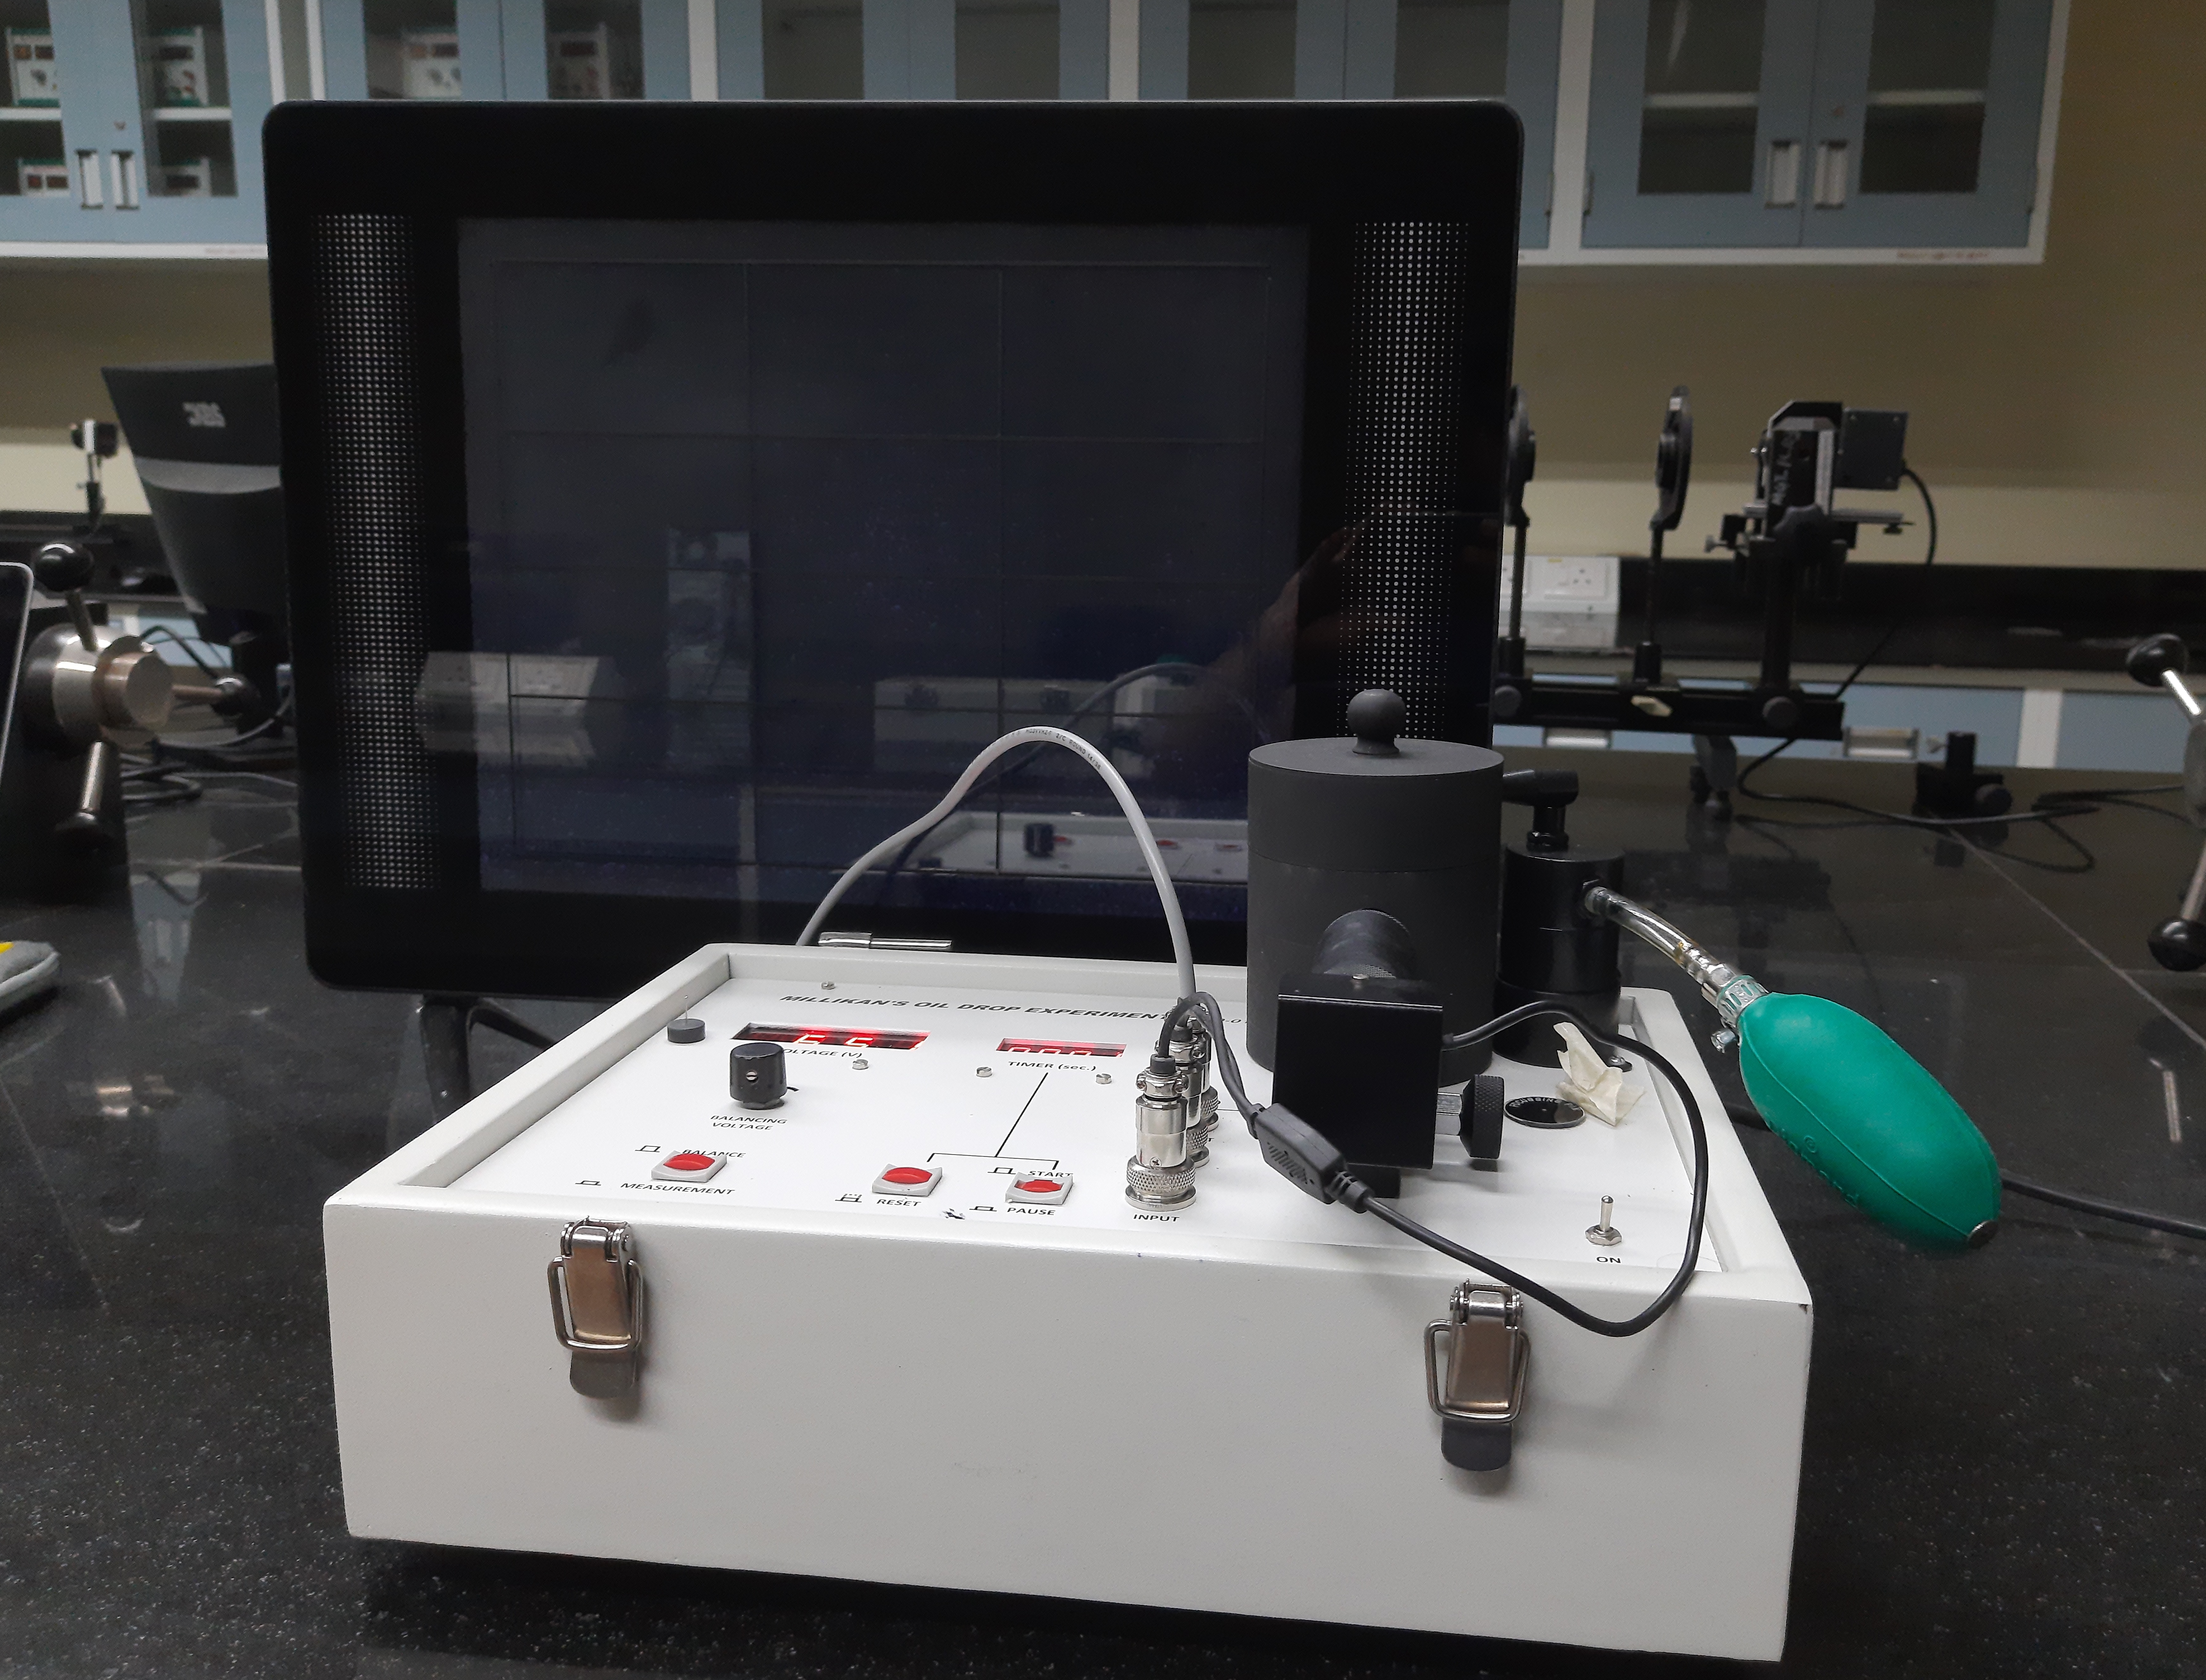
\includegraphics[width=8.3cm,height=6cm]{1} 
	\caption{Experimental setup in laboratory}
	\label{1}
\end{figure}

\subsection{Precautions}
\begin{enumerate}
	\item {Place the setup in very flat place free from mechanical disturbances.}
	\item {Always focus on the right droplet to avoid losing it.}
	\item{Select appropriately sized droplets, neither too large nor small.}
	\item{Do not spray large amounts of droplets into the plates. }
\end{enumerate}


\section{Observation and Analysis}
Distance between parallel plates, d =$0.5 cm$\newline
Distance between two lines on monitor, L =$0.1 cm$\newline
Density of oil, $\rho$=$929kg/m^3$\newline
Density of air, $\rho_a$=$1kg/m^3$\newline
Room temperature, T=24$^\circ$C\newline
Atmospheric pressure P= 0.76 mHg\newline
Coefficient of viscosity of air, $\eta$=1.8$\times$ $10^{-5}$ kg/msec\newline

\begin{figure}[H] %  figure placement: here, top, bottom, or page
	\centering
	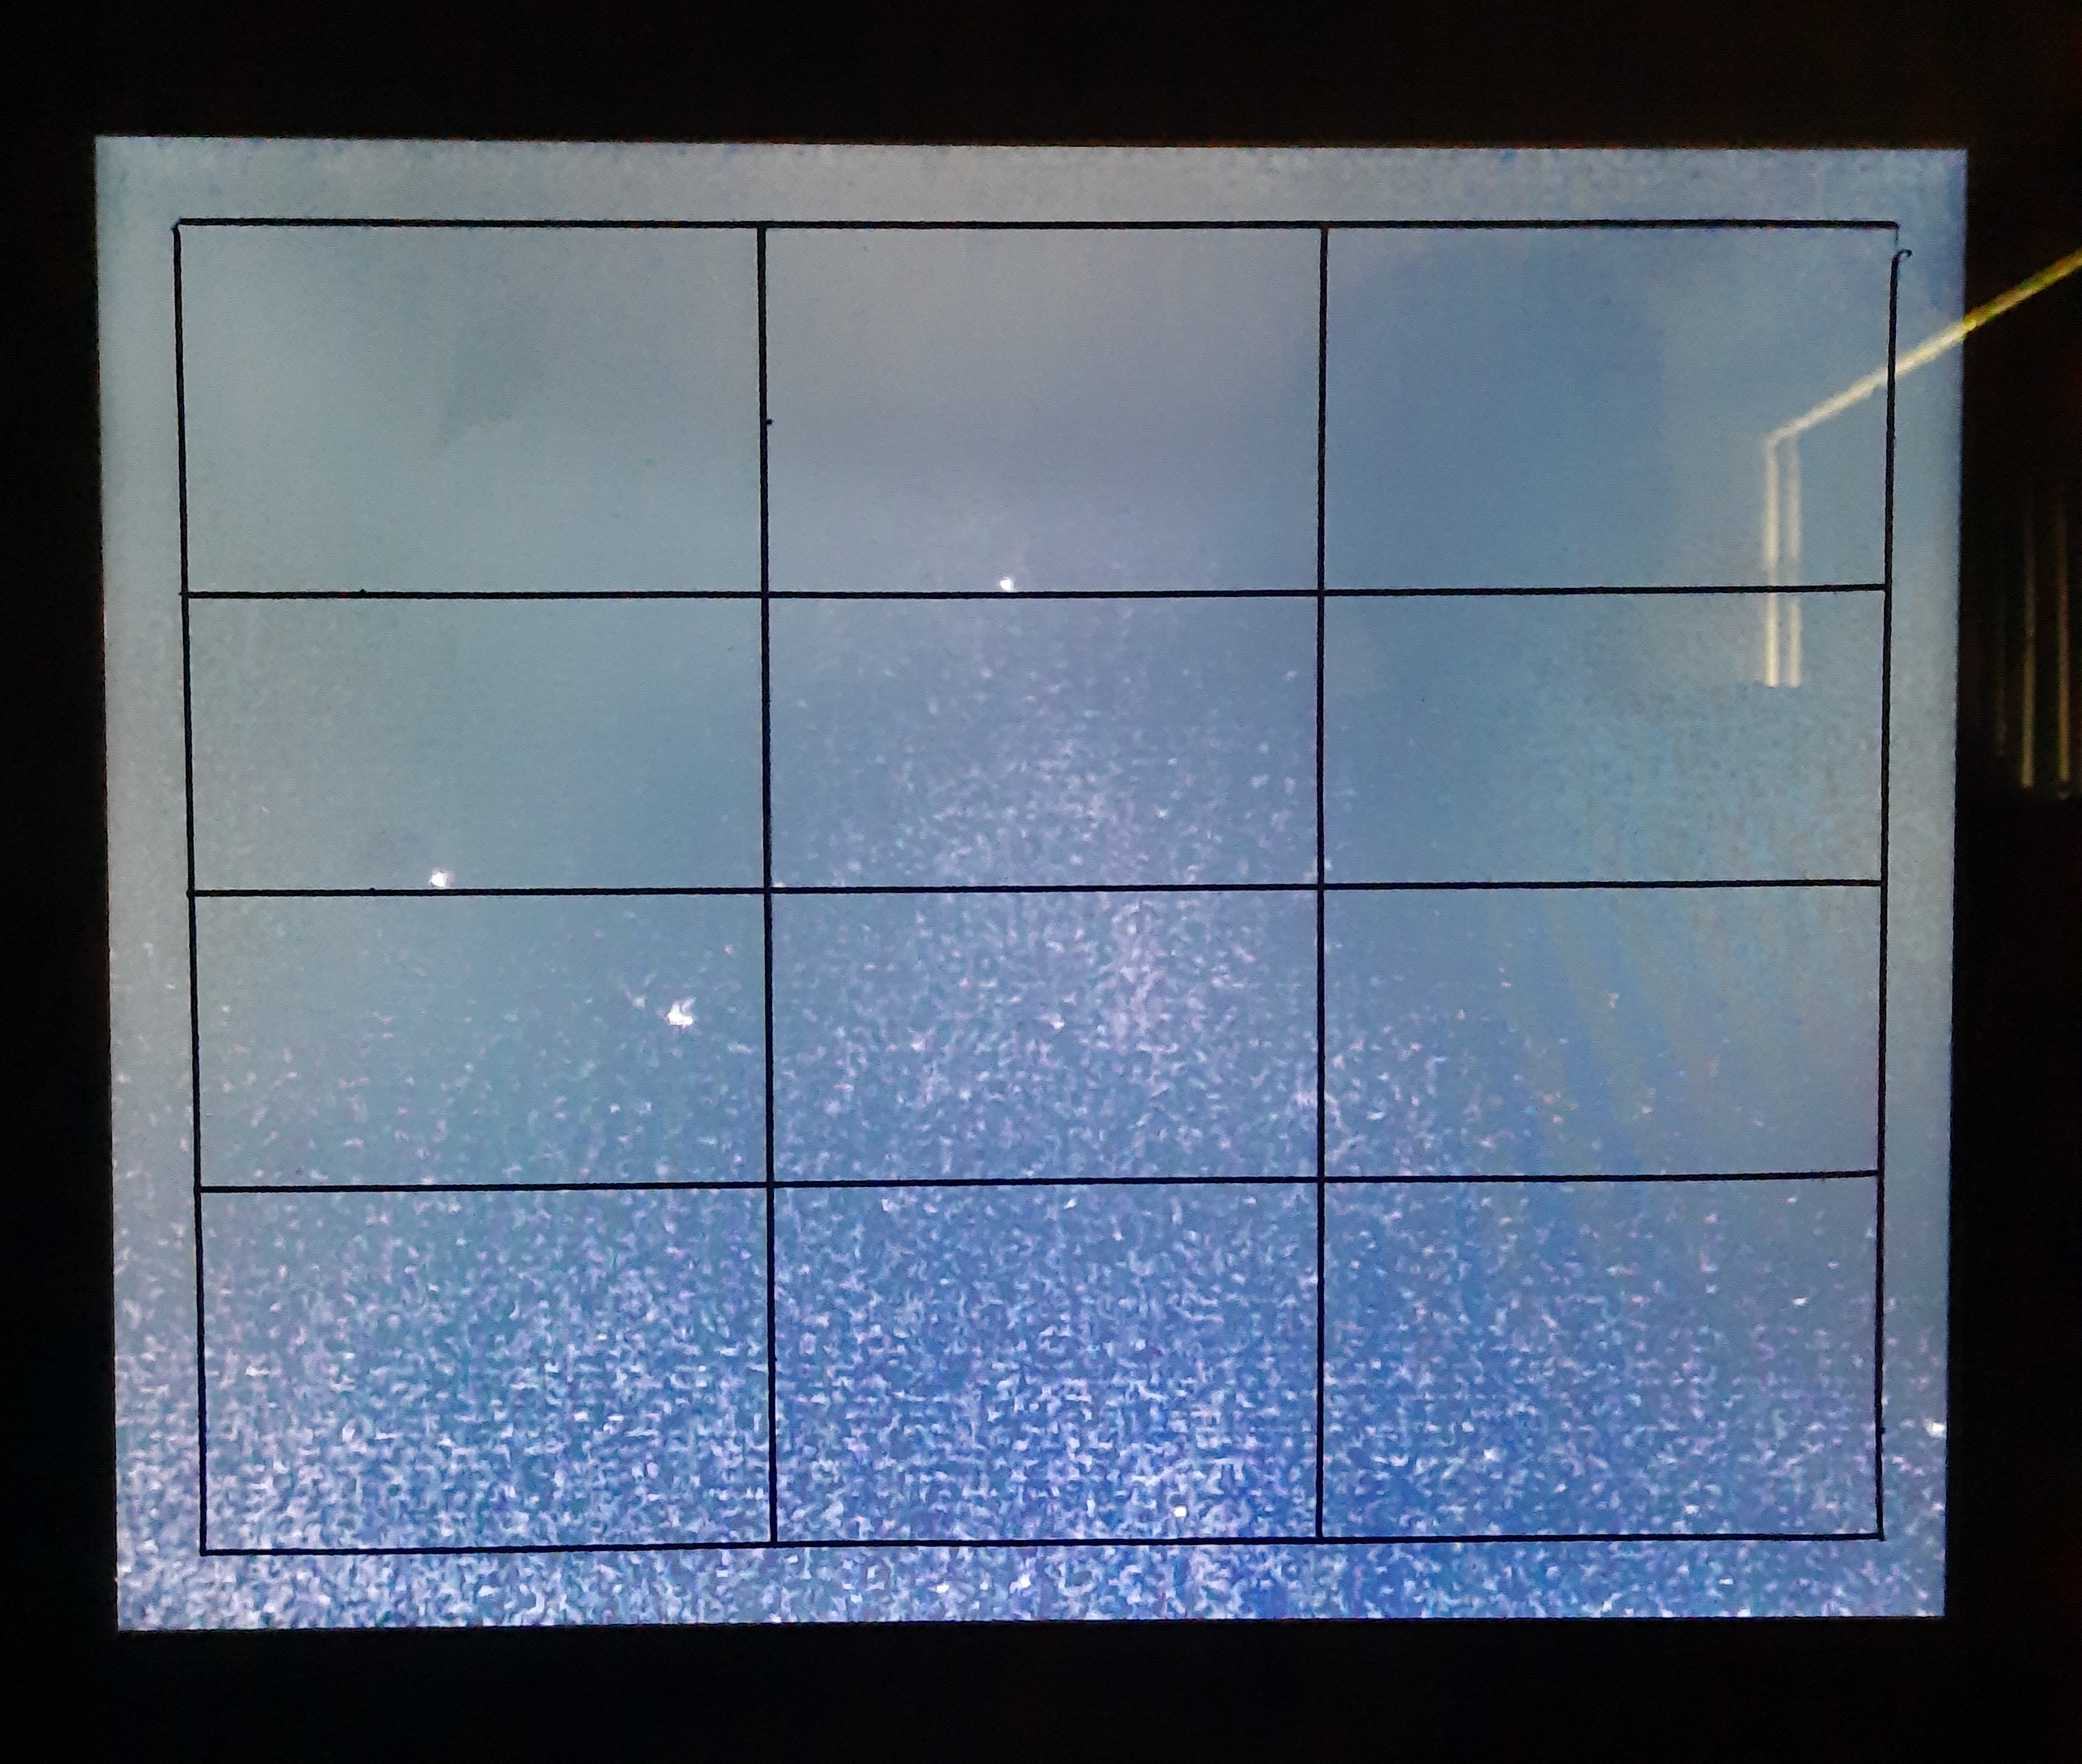
\includegraphics[width=8.3cm,height=6cm]{2} 
	\caption{Oil droplets (white dots) as seen on LCD screen. }
	\label{2}
\end{figure}

The readings and calculations for dynamic and balancing method are attached with this report. Kindly refer to that.

For dynamic method,
Error in charge of electron, e is calculated as below, with r$\propto$ $\xi^{0.5}$
\begin{equation}
	\frac{\delta r}{r}= \left(\frac{1.\delta t_f}{2.t_f}\right)=\frac{0.1}{2\times12.953}=3.86\times10^{-3}
\end{equation}

\begin{equation}
	\frac{\delta T}{T}=\sqrt{ \left(\frac{\delta t_f}{t_f}\right)^2+\left(\frac{\delta t_r}{t_r}\right)^2}=\sqrt{ \left(\frac{0.1}{12.953}\right)^2+\left(\frac{0.1}{6.783}\right)^2}
\end{equation}

\begin{equation}
	\frac{\delta T}{T}=1.66\times10^{-2}
\end{equation}

\begin{equation}
	\frac{\delta e}{e}=\sqrt{ \left(\frac{\delta T}{T}\right)^2+\left(\frac{3.\delta r}{r}\right)^2}
\end{equation}

\begin{equation}
	\frac{\delta e}{4.706\times10^{-19}}=\sqrt{ \left(1.66\times10^{-2}\right)^2+\left(3.\times3.86\times10^{-3}\right)^2}
\end{equation}

giving $\delta e$ as $0.095\times10^{-19} C.$
\newline
\newline
Similarly for the case balancing method, 
\begin{equation}
	\frac{\delta r}{r}= \left(\frac{1.\delta t_f}{2.t_f}\right)=\frac{0.1}{2\times11.026}=4.53\times10^{-3}
\end{equation}

\begin{equation}
	\frac{\delta e}{e}= \left(\frac{3.\delta r}{r}\right)\implies \delta e =0.028\times10^{-19} C
\end{equation}

In the above formulae, the normal notations are equivalent to average of those symbols, example, $T$ is $T_{avg}$

\section{Conclusion and Summary}

From this experiment, we tried to calculate the charge of electron by two methods, dynamic method and balancing method. In dynamic method the oil droplet is allowed free fall and then allowed to rise in electric field; by calculating the time taken to rise and fall, we can determine the charge on electron with the working formula derived from various forces such as buoyant force, gravitational force, electric force, viscous force etc.. acting on the droplet during this process. In case of balancing method, the droplet is kept stationary with the help of certain potential difference to cancel out other forces acting on it. The fall time is also noted to determine the charge of electron. 

From dynamic method, we found charge of electron as $(4.706\pm0.095)\times10^{-19} C$ and with balancing method we found charge of electron as $(2.076\pm0.028)\times10^{-19} C$. The actual value of charge of electron is $1.602\times10^{-19} C$. It is evident that the error in first method is very large with percentage error as 193.76\% and in second method, percentage error was calculated to be 29.58\%.

The errors in the experiment arises due to instrumental artifacts such as fluctuating voltage between the two plates. Moreover choice of droplet plays an important game for this experiment. Drops with varying size was considered resulting in larger range of fall and rise time, hence deviating from the original value. Some random errors as well as human errors while measuring fall and rise time, also contributed to such deviation. The user may have lost the droplet while measuring the time count. The balancing method proves to be relatively better than the dynamic method in our experiment as we got acquainted with the setup, the size of the droplet, accuracy was better. Hence, in our case, for this experiment, balancing method gave better value of charge on electron.


\section{References}
\begin{enumerate}
\item {\url{https://www.niser.ac.in/sps/sites/default/files/basic_page/Milican's%20Oil%20Drop%20Experiment.pdf}}
\end{enumerate}

\end{document}